%%=============================================================================
%% Methodologie
%%=============================================================================

\chapter{\IfLanguageName{dutch}{Methodologie}{Methodology}}
\label{ch:methodologie}

Binnen dit hoofdstuk zal het experiment verder worden toegelicht.

In sectie \ref{sec:opzet} zal er worden stilgestaan bij de opzet van het experiment en hoe de platformen geëvalueerd zijn.

In sectie \ref{sec:dataset} wordt er meer uitleg voorzien rond het testscenario en de opgestelde dataset

In sectie \ref{sec:validatie} wordt er toegelicht hoe de platformen op een objectieve manier geëvalueerd en vergeleken worden.

In sectie \ref{sec:werking-platformen} wordt er meer uitleg gegeven bij de werking van de verschillende platformen. Daarbij wordt stilgestaan bij creëren van een chatbot, het toevoegen van intents, het trainen met voorbeeldzinnen en hoe de gebouwde chatbots getest kunnen worden

In sectie \ref{sec:automatisatie} zal ten slotte meer informatie worden gegeven rond de praktische implementatie van het experiment en hoe het trainen en testen van de platformen geautomatiseerd wordt.


\section{Opzet}
\label{sec:opzet}

Om een vergelijking te kunnen maken van het begrijpend vermogen van de platformen, moet er een experiment plaatsvinden waarbij er op een objectieve manier beoordeeld kan worden. Daarom is er een dataset opgesteld waarmee alle platformen zullen getraind en geëvalueerd worden. Op deze manier krijgen alle platformen exact evenveel informatie en kan er objectief geoordeeld worden. Een deel van de dataset zal gebruikt worden voor het trainen en het andere deel zal dienen voor het testen. Deze dataset zal bestaan uit een aantal intents met bijbehorende voorbeeldzinnen die bij dat bepaalde intent horen. Op deze manier kunnen de ML algoritmes modellen bouwen om de juiste intent te herkennen als een gebruiker een bericht naar de chatbot stuurt. Indien intents geen voorbeeldzinnen krijgen, dan zal het trainen onmogelijk zijn, wat een sterke invloed zal hebben op de accuraatheid. De meeste platformen vereisten een minimum van 5 voorbeeldzinnen om het trainen te kunnen starten, maar het is sterk aangewezen om minimum 10-15 voorbeeldzinnen per intent te voorzien \autocite{Greyling2019}. Eens het trainen gedaan is, kan het valideren beginnen. Het is de bedoeling om uiteindelijk een platform aan te duiden die het beste begrijpend vermogen heeft en dus het beste presteert op het herkennen van de juiste intent. Daarbij zal op 3 verschillende manieren geëvalueerd worden. Het hoofddoel van dit onderzoek is om te bepalen welk platform het beste presteert op intent herkenning. Daarbij wordt er beoordeeld op de prestaties bij zowel het gebruik met als het gebruik zonder entities. Het is algemeen aangeraden om entities te gebruiken, maar in dit onderzoek wordt er ook gekeken naar de invloed op de resultaten als er entities worden gebruikt in tegenstelling tot het weglaten van entities. Daarnaast wordt er ook beoordeeld op hoe goed de getrainde applicaties om kunnen gaan met taalvariaties. Gebruikers schrijven vaak niet in het standaard nederlands als ze communiceren via het internet, daarom wordt er verwacht dat ze dit ook niet zullen doen als ze praten met een chatbot. Daarom is het belangrijk dat een chatbot ook de intentie van berichten zo goed mogelijk kan verstaan als gebruikers afkortingen, slecht gevormde woorden en zinnen en dialecten gebruiken.

%TODO informatie rondom alles van de entities toevoegen hier
\section{Dataset}
\label{sec:dataset}

De dataset is opgesteld op basis van een fictieve use case die werd bepaald in samenwerking met de co-promotor. Het is de bedoeling om een virtuele assistent te bouwen voor een busreisorganisatie. Het bedrijf wil mee met de digitale evolutie en wil gebruikers de mogelijkheid te geven om interactie aan te gaan met een geautomatiseerde gesprekspartner om informatie te krijgen, busreizen te boeken en te beheren en om eventuele klachten af te handelen. Daarbij zijn er een aantal intents gedefinieerd.

Er werd gekozen voor de volgende intents:
\begin{itemize}
    \item greetings
    \item geefBestemmingen
    \item geefReisTijden
    \item boekBusreis
    \item geefActueleInfo
    \item wijzigBusreis
    \item annuleerBusreis
    \item geefOnboardServices
    \item meldKlachten
    \item huurBusMetChauffeur
\end{itemize}

\textbf{Hier moet nog informatie rondom de gekozen entities komen}

Elk van deze intents werd voorzien met 15 voorbeeldzinnen. Bij het opstellen is het belangrijk dat er rekening wordt gehouden met een aantal zaken \autocite{Greyling2019}:
\begin{itemize}
    \item Gebruik korte en lange zinnen
    \item Verschillende synoniemen gebruiken
    \item Varieer de positie van entities
    \item Wissel grammatica af
    \item Gebruik woorden zowel in enkelvoud als in meervoud
    \item Gebruik niet altijd hoofdletters en leestekens
\end{itemize}

\section{Validatie}
\label{sec:validatie}

Chatbots zijn voorbeelden van gesuperviseerd leren, daarbij is het de bedoeling dat er op basis van trainingsdata modellen worden opgesteld die voor ongekende input de correcte output kunnen voorspellen. Dit zal ook binnen dit experiment worden toegepast. Er zijn 15 voorbeeldzinnen voorzien per intent en het is de bedoeling dat er een deel van deze zinnen worden gebruikt om de chatbots te trainen en dat het resterende deel wordt gebruikt als input om te valideren dat het model wel de juiste intent kan herkennen.

De meest gebruikte methode is om 80\% van de data te gebruiken om te trainen en dat de resterende 20\% wordt gebruikt om te testen \autocite{Desmarais2018}. Deze methode is eenvoudig te implementeren, maar het probleem hierbij is dat bepaalde data niet wordt gebruikt om te trainen en dat andere data niet wordt gebruikt om te testen. Dat kan resulteren in minder accurate resultaten.

De oplossing voor dit probleem is K-Fold Cross Validation \autocite{Desmarais2018}. Hierbij wordt de dataset in een aantal gelijke delen verdeeld en wordt er één deel gebruikt voor het testen, waarbij de resterende delen worden gebruikt om te trainen. Dit wordt een aantal keer herhaald, afhankelijk van het aantal delen dat je hebt gekozen, dat zijn het aantal cycli die doorlopen worden. Het meest gebruikte aantal delen is 5, omdat er op deze manier ook aan het 80/20 principe kan voldaan worden. vier delen worden dan gebruikt om de chatbot te trainen (80\%) en het andere deel voor te valideren (20\%). Bij een volgende cyclus wordt er dan doorgeschoven. Het grote voordeel van deze methode is dat het veel betrouwbaarder en robuuster is, omdat er 5 keer zoveel tests zijn dan bij de andere methode en ook omdat alle data gebruikt wordt voor zowel trainen als testen.

\begin{figure}[H]
    \label{fig:cross-validation-schema}
    \centering
    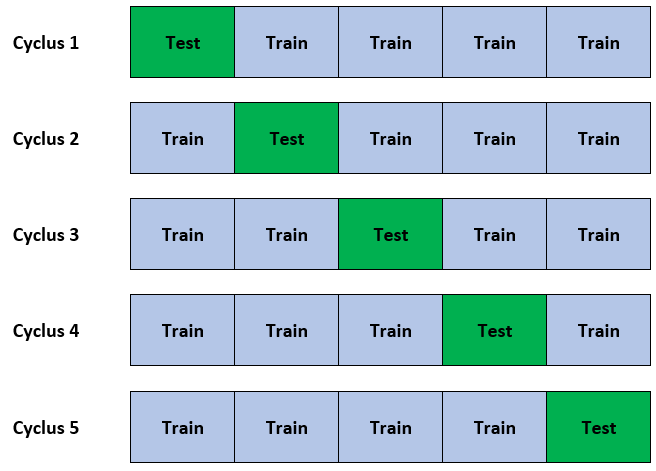
\includegraphics[width=0.85\textwidth]{schema-cross-validation}
    \caption{Grafische voorstelling van de werking van cross validation}
\end{figure}

\subsection{Confusion matrix}
\label{subsec:validatie-confusion-matrix}

Een confusion matrix is een heel erg duidelijk representatie van de resultaten van een classificatieprobleem die in dit onderzoek gebruikt wordt. Het is een overzicht van hoeveel keer een categorie voorspeld werd en hoeveel keer dit juist of fout is. Het is ook duidelijk zichtbaar welke categorie werd gekozen indien dit niet correct is. Vanuit een confusion matrix kunnen ook interessante metrieken berekend worden. Berekeningen kunnen worden gedaan per categorie of in het geheel. Een voorbeeld van een confusion matrix voor een classificatieprobleem wordt geïllustreerd in onderstaande afbeelding.

\begin{figure}[H]
    \label{fig:confusion-matrix-voorbeeld}
    \centering
    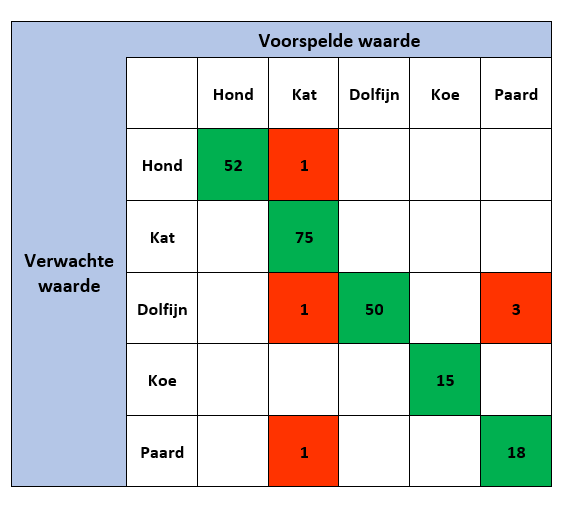
\includegraphics[width=0.85\textwidth]{confusion-matrix-voorbeeld}
    \caption{Voorbeeld van een confusion matrix}
\end{figure}

De linkerkant (de rijen) staan voor het dier die verwacht wordt en de kolommen staan voor het dier die voorspeld is. Hieruit kunnen bepaalde conclusies genomen worden, hier een aantal voorbeelden:
\begin{itemize}
    \item Er zijn 53 (52+1) gevallen waarbij een hond verwacht wordt, bij 52 gevallen werd dit ook effectief voorspeld door het model. Eén keer werd een fout dier voorspeld (kat).
    \item De dieren kat en koe werden altijd voorspeld als ze verwacht werden.
    \item De dieren hond, dolfijn en koe werden nooit voorspeld als ze niet verwacht werden.
\end{itemize}

\subsection{Precision, Recall \& F-score}
\label{subsec:validatie-precision-recall-f-score}

Er zijn een aantal interessante metrieken die kunnen berekend worden uit een confusion matrix. Deze worden gebruikt om platformen met elkaar te vergelijken. Al deze metrieken kunnen zowel berekend worden per intent/categorie, als in het geheel.

\subsubsection{Precision}

Precision is een metriek die aangeeft in hoeveel procent van de gevallen dat de voorspelde waarde ook effectief de juiste blijkt te zijn.
In bovenstaand voorbeeld kan er worden afgeleid dat een paard 21 (18+3) keer werd voorspeld. In 18 van de gevallen blijkt dit ook correct te zijn. Dat betekend dat de precision van deze categorie ~ 86% (18/21) is. 

\subsubsection{Recall}

Recall is een andere metriek die aangeeft hoeveel procent van de categorieën correct voorspeld zijn. In bovenstaand voorbeeld zijn er 19 (18+1) voorbeelden waarbij een paard verwacht wordt. In 18 gevallen werd het juiste dier herkent. Dat betekend dat de recall voor deze categorie~ 95\% (18/19) is.

Initieel lijken de metrieken precision en recall sterk op elkaar, maar toch zijn ze volledig verschillend van elkaar, dat bewijst het voorbeeld.

\subsubsection{F-score}

Precision en recall op zich vertellen niet veel over de kwaliteit van het model \autocite{Treml2019}. Ze zijn enkel nuttig indien je zowel de precision als de recall kent. Om dit wat samen te gieten in één duidelijke metriek, bestaat er zoiets als de f-score. Dat is het harmonisch gemiddelde van de recall en de precision. De f-score verteld hoe kwalitatief een classificatiemodel is. Hoe hoger de f-score, hoe beter. Binnen dit onderzoek wordt vooral de f-score gebruikt om de resultaten van platformen met elkaar te vergelijken.

De f-score (harmonisch gemiddelde) bereken je als volgt:
\begin{itemize}
    \item $F= 2 * \frac{precision*recall}{precision+recall}\\$
\end{itemize}

In het geval van een paard is de f-score ongeveer gelijk aan 90\%.


\section{Werking van de platformen}
\label{sec:werking-platformen}


In deze sectie zal worden toegelicht hoe de verschillende platformen functioneren. Dit is een belangrijk onderdeel binnen dit onderzoek. Er zal stilgestaan worden bij het creëren van een chatbot, het toevoegen van intents, het trainen met voorbeeldzinnen en hoe de gebouwde chatbots getest kunnen worden. Binnen deze sectie zullen ook functionaliteiten van platformen worden toegelicht die niet gebruikt zijn voor het experiment. Dit experiment focust zich op het classificeren van intents en niet op een volledige conversatie met de chatbot, maar het is wel belangrijk om stil te staan bij de mogelijkheden van elk platform om een volledige conversatie te voeren.

\subsection{Dialogflow}
\label{subsec:werking-platformen-dialogflow}

Dialogflow is een heel erg gebruiksvriendelijk platform die zowel voor technische als geen technische mensen verstaanbaar en te gebruiken is. Het helpt natuurlijk wel als je enige technische kennis hebt om alles vlotter te verstaan. Het enige die nodig is om aan de slag te gaan met Dialogflow is een Google account. Iedereen kan er mee aan de slag omdat het grotendeels gratis is De betaalde versie is eerder voor bedrijven die complexe chatbots willen opzetten en veel gebruikers zullen hebben. Doordat het onderdeel is van Google Cloud Platform, kan er ook makkelijk gebruik gemaakt worden van de diverse google services die beschikbaar zijn. Er zijn ook vele analysemogelijkheden aanwezig die gebruikt kunnen worden om prestaties te monitoren. Dialogflow gebruikt de term agenten (agents) voor hun chatbots. Dat doen ze omdat ze de vergelijking willen maken met menselijke call center agenten \autocite{GoogleCloud2020}. Agenten verwerken conversaties met eindgebruikers. Er zijn ook heel wat voorgebouwde agenten beschikbaar die gratis gebruikt kunnen worden. Bij het maken van een agent moet een naam opgegeven worden en moet er een standaardtaal gekozen worden. Het is mogelijk om extra talen toe te voegen indien er een meertalige agent gebouwd moet worden. Het is ook mogelijk om de agent te linken aan een Google Cloud project, op die manier is de samenwerking met andere services eenvoudiger. 

\begin{figure}[H]
    \label{fig:dialogflow-create}
    \centering
    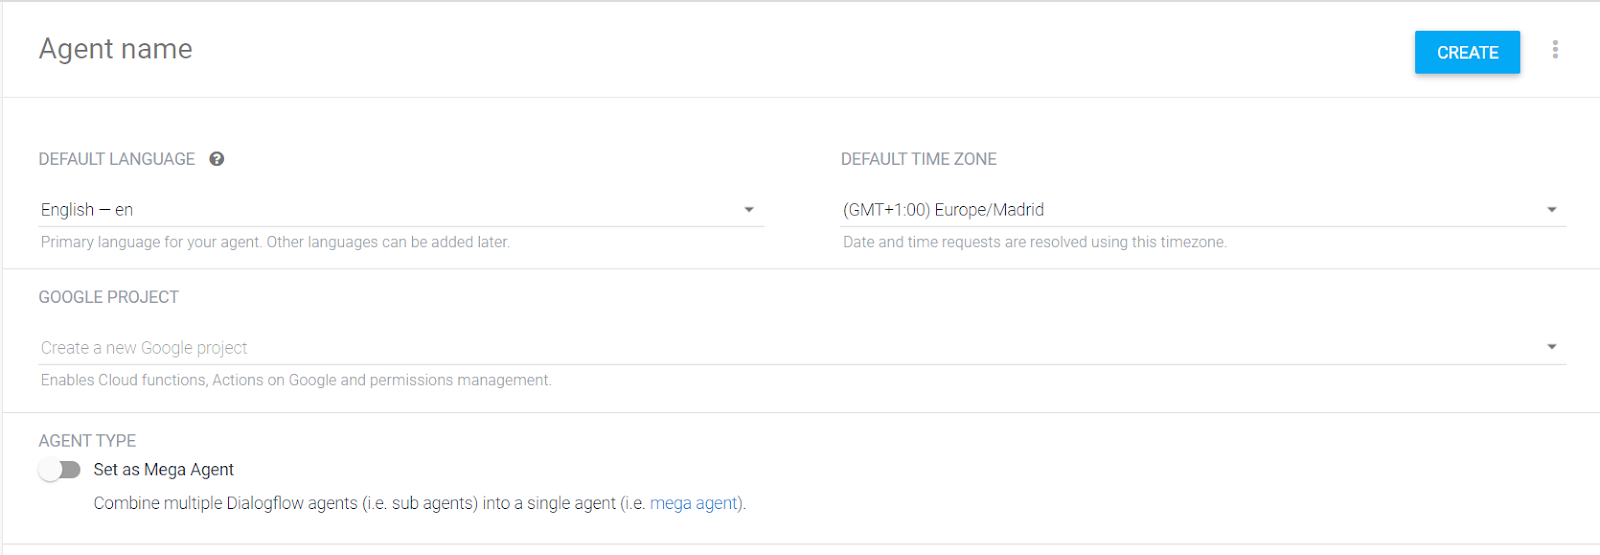
\includegraphics[width=\textwidth]{dialogflow-create}
    \caption{Het creëren van een agent in Dialogflow}
\end{figure}

Agenten gebruiken intents om de intentie van berichten die gebruikers sturen te achterhalen. Bij het toevoegen en configureren van intents moet er een naam opgegeven worden en kunnen er diverse trainingszinnen toegevoegd worden. Dialogflow vereist een minimum van 5 voorbeeldzinnen per intent. Het is ook mogelijk om bij voorbeeldzinnen entities/parameters toe te voegen. Er zijn heel wat entities ingebouwd in het systeem die ook allemaal gratis gebruikt kunnen worden. Per intent kunnen er ook antwoorden voorzien worden die de agent stuurt als die intent geclassificeerd wordt. Er is ook de mogelijkheid om events toe te voegen die dan deze intent gaan uitvoeren zonder dat het getriggerd moet worden door tekst of spraak.

\begin{figure}[H]
    \label{fig:dialogflow-intent}
    \centering
    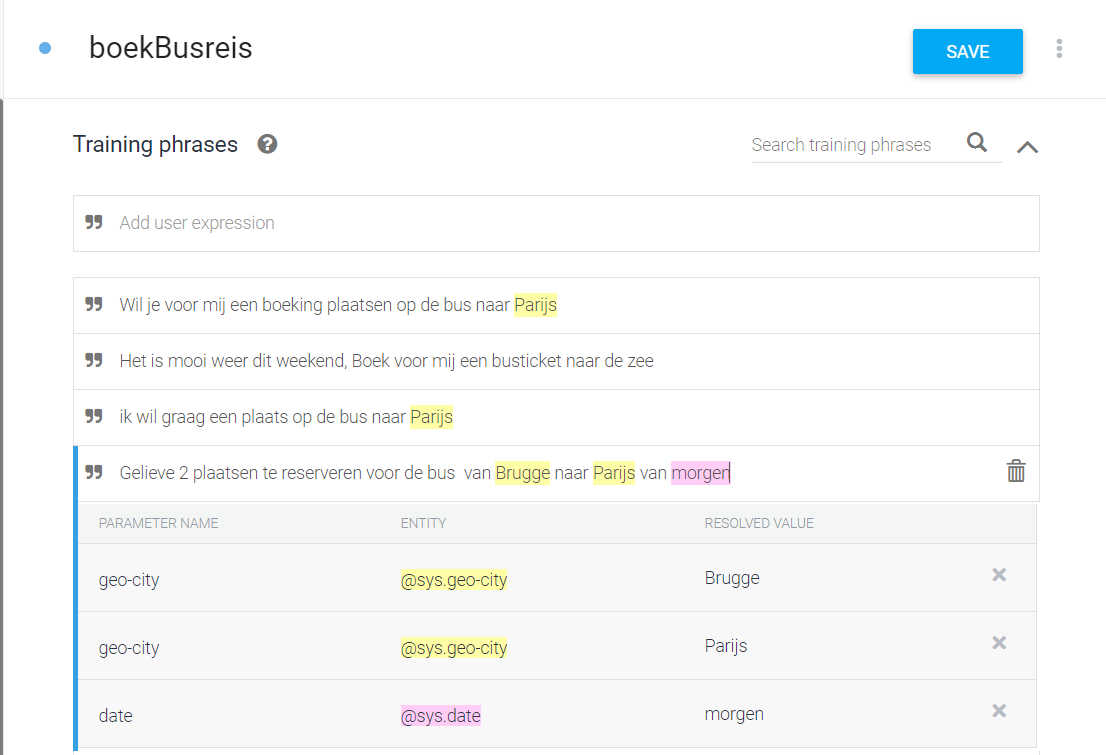
\includegraphics[width=\textwidth]{dialogflow-intent}
    \caption{Het toevoegen van voorbeeldzinnen en het aanduiden van de entities in een intent in Dialogflow}
\end{figure}

Het is ook mogelijk om contexten toe te voegen aan intents, dat wordt gebruikt om parameterwaarden bij te houden gedurende conversaties. Op die manier moet de chatbot geen informatie vragen aan de gebruiker die hij eigenlijk al heeft gekregen. Dat maakt de gebruikerservaring een stuk aangenamer. Contexten zullen in deze bachelorproef niet verder worden gebruikt, maar het is wel interessant dat Dialogflow dit heeft.

\begin{figure}[H]
    \label{fig:dialogflow-context}
    \centering
    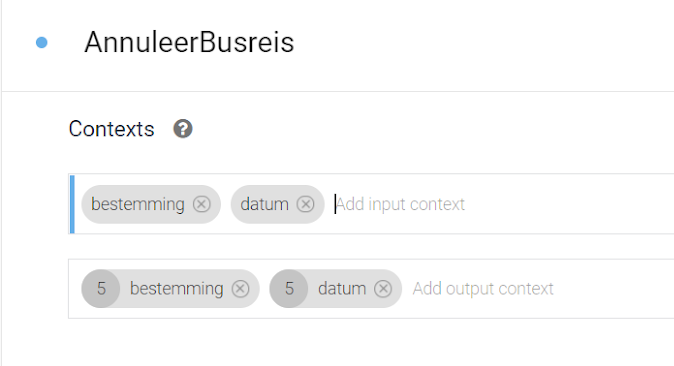
\includegraphics[width=0.7\textwidth]{dialogflow-context}
    \caption{Het toevoegen van contexten in een intent in Dialogflow}
\end{figure}

Aangezien er heel wat systeementiteiten zijn voorzien in Dialogflow, kan het zijn dat het niet meteen nodig is om zelf entities aan te maken, maar het is wel mogelijk. Bij het aanmaken van een entiteit kunnen verschillende waarden toegevoegd worden om de agent deze entiteit te doen herkennen bij user input. Er kunnen synoniemen gegeven worden en er is ook de mogelijkheid om een specifiek patroon op te geven waarvoor een entiteit herkent wordt in zinnen. De gemaakte entiteiten kunnen dan net zoals systeementiteiten toegevoegd worden aan voorbeeldzinnen in de intents.

\begin{figure}[H]
    \label{fig:dialogflow-entity}
    \centering
    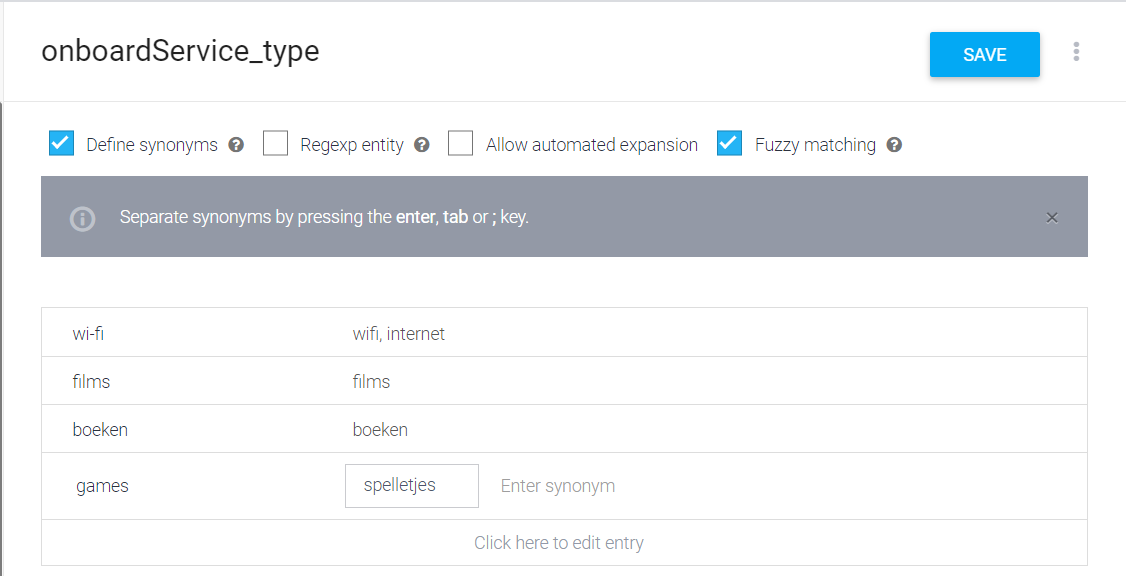
\includegraphics[width=\textwidth]{dialogflow-entity}
    \caption{Het aanmaken en beheren van een entity in Dialogflow}
\end{figure}

Met Dialogflow is het ook mogelijk om voorgaande berichten van eindgebruikers te valideren, zodat die dan gebruikt kunnen worden als extra voorbeeldzinnen bij de intents. Op deze manier wordt de agent steeds slimmer doorheen zijn levensloop. Het is ook mogelijk om een intent classificatie te weigeren en ook om de herkende intent te wijzigen en toch goed te keuren. 

\begin{figure}[H]
    \label{fig:dialogflow-validate}
    \centering
    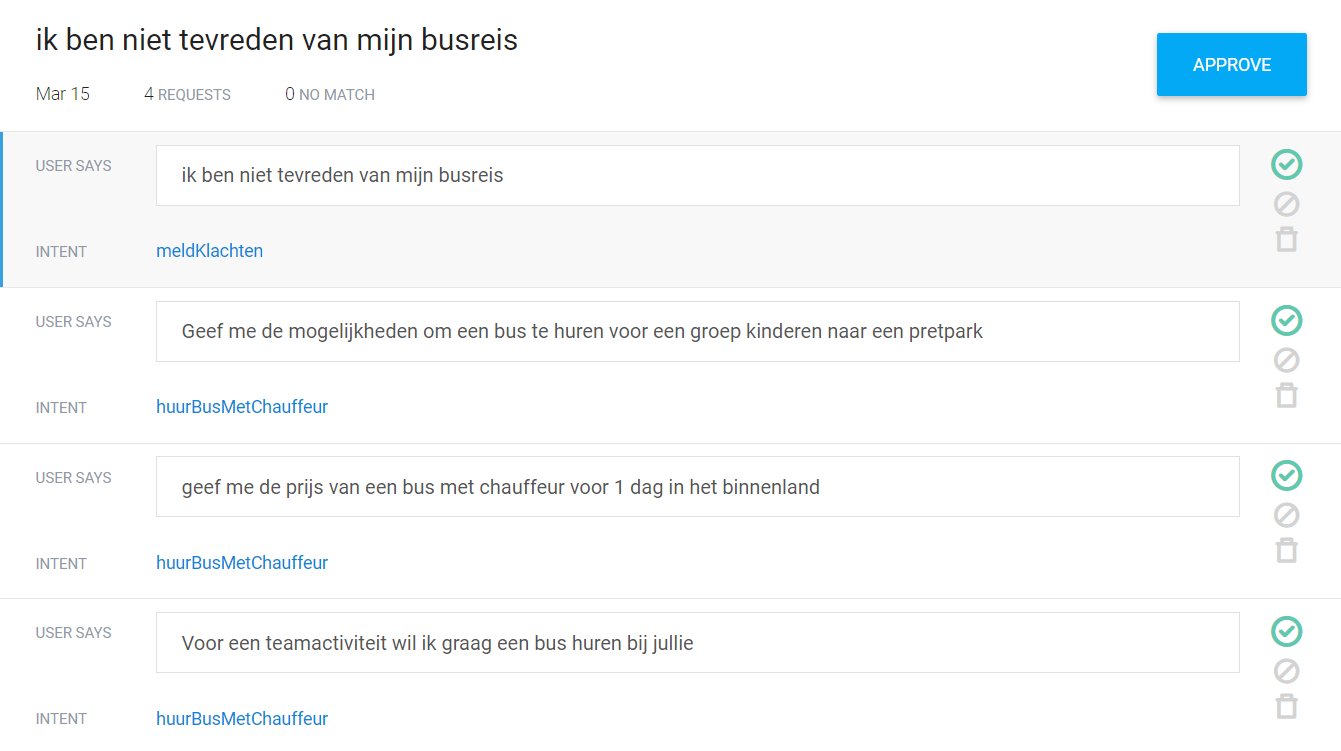
\includegraphics[width=\textwidth]{dialogflow-validate}
    \caption{Het valideren van user input om het model uit te breiden in Dialogflow}
\end{figure}

Dialogflow is heel erg makkelijk te integreren met andere diensten. Het enige dat je als ontwikkelaar moet doen is de integratie aanzetten en dan komt er informatie beschikbaar die uitlegt wat je precies moet doen om het te activeren. Het is ook mogelijk om zelf een applicatie te schrijven die gebruik maakt van de API van Dialogflow.

De chatbot testen kan ook via de user interface (UI) gebeuren. Dit kan worden gedaan door een bericht te sturen naar de ingebouwde conversatiemodule. Bij het sturen van een bericht krijg je informatie over welke intent is herkent, wat het antwoord is en welke actie eventueel uitgevoerd werd. Het is ook mogelijk om meer gedetailleerde resultaten te zien. Opnieuw zal er in deze bachelorproef geen speciale aandacht besteed worden aan het antwoorden naar gebruikers.

\begin{figure}[H]
    \label{fig:dialogflow-test}
    \centering
    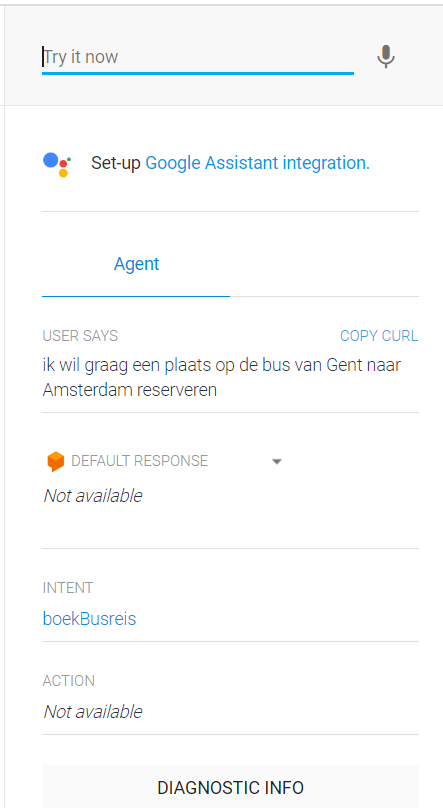
\includegraphics[width=0.5\textwidth]{dialogflow-test}
    \caption{Het testen van de agent met de conversatiemodule in Dialogflow}
\end{figure}

\subsection{IBM Watson}
\label{subsec:werking-platformen-ibm-watson}

IBM watson is het chatbotplatform die ontwikkeld is door IBM. Het is een onderdeel van IBM cloud en zeer goed vergelijkbaar met Google Cloud. Ze bieden ongeveer dezelfde functionaliteiten aan. Om een chatbot op te zetten heb je enkel een IBM Cloud account nodig. IBM Watson is gekend voor zijn zeer gebruiksvriendelijke grafische user interface (GUI) en voor de snelheid waarmee een chatbot ontwikkeld kan worden. IBM Watson biedt ook analysemogelijkheden aan op hun chatbotplatform en gebruikt de naam assistent voor zijn chatbots. het aanmaken van een assistent is heel erg eenvoudig. Een naam en een beschrijving is het enige die gevraagd wordt op een assistent aan te maken.

\begin{figure}[H]
    \label{fig:watson-create}
    \centering
    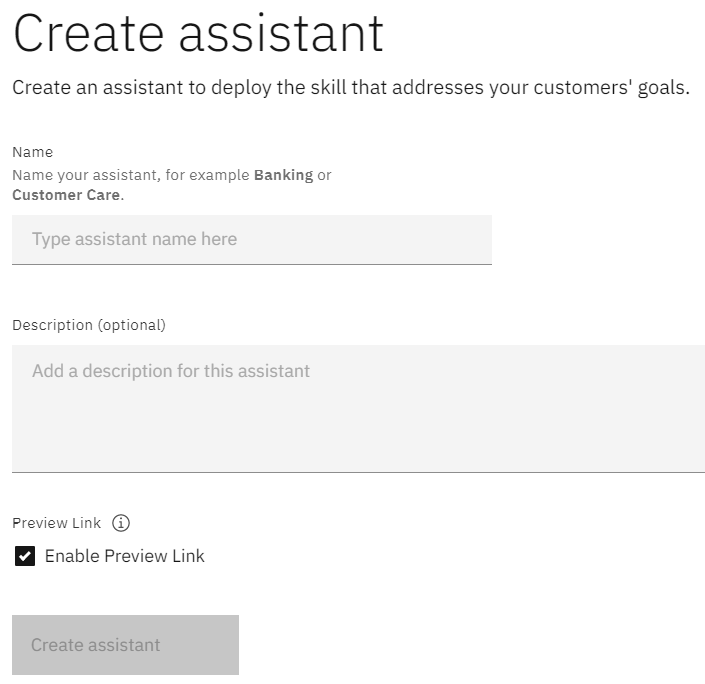
\includegraphics[width=0.75\textwidth]{watson-create}
    \caption{Het aanmaken van een assistent in IBM Watson}
\end{figure}

IBM werkt voor het trainen van zijn assistenten met zogenaamde skills. Een skill bevat alles om klantenaanvragen te beantwoorden. Het is niet zo dat er bij IBM Watson assistent per assistent wordt getraind, maar er wordt een skill aangemaakt die dan kan toegevoegd worden aan de assistent naar keuze. Er kunnen dus meerdere skills aan één assistent toegevoegd worden. Bij het aanmaken van een skill is het noodzakelijk om een naam en een standaardtaal op te geven. Door verschillende skills met verschillende talen toe te voegen aan een assistent kan er dus ook een meertalige assistent gemaakt worden.

\begin{figure}[H]
    \label{fig:watson-skill}
    \centering
    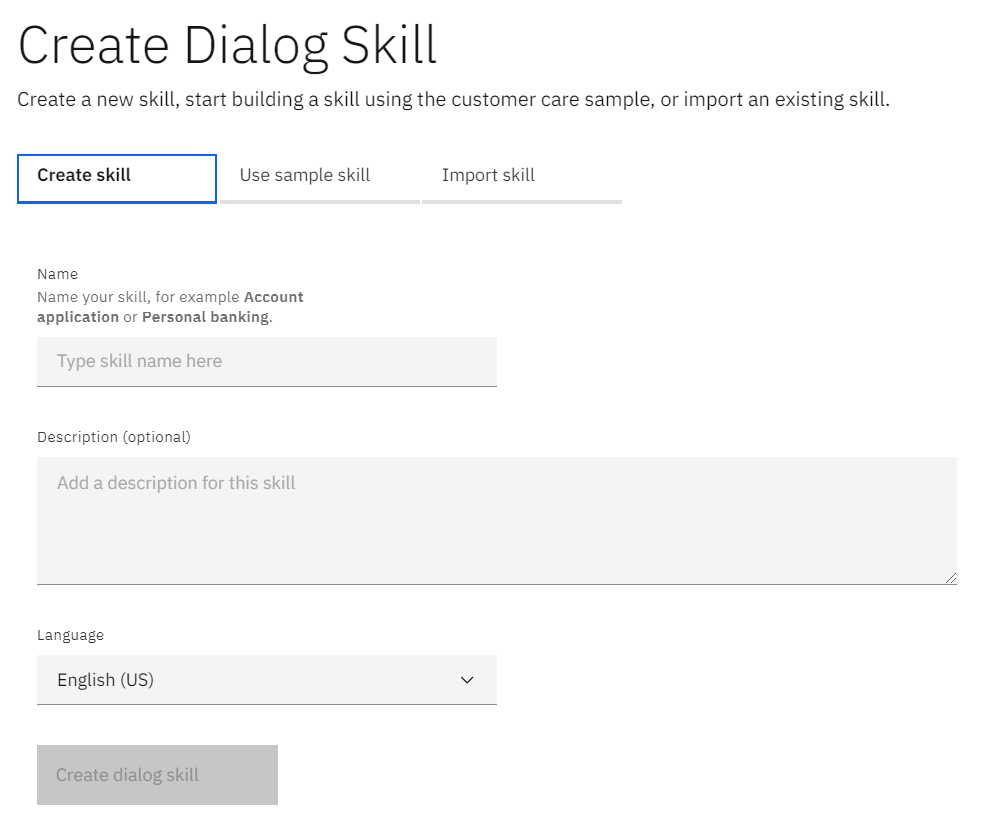
\includegraphics[width=0.75\textwidth]{watson-skill}
    \caption{Het aanmaken van een skill in IBM Watson}
\end{figure}

Eens een skill is aangemaakt, kan het configureren van de skill beginnen. Het toevoegen van een intent is opnieuw heel erg eenvoudig. Een naam en een aantal voorbeeldzinnen is alles die nodig is. IBM Watson legt geen restricties op het aantal voorbeeldzinnen, maar opnieuw is het aangeraden om er toch 10-15 te voorzien per intent. Het configureren van intents verschilt ook met de andere platformen, omdat er geen entities toegevoegd kunnen worden aan de intents en aan de voorbeeldzinnen. Dat is een andere functionaliteit die IBM met hun chatbot platform achter de schermen gaat doen voor de ontwikkelaar. Watson gaat zelf op zoek naar entiteiten in de voorbeeldzinnen zonder dat de ontwikkelaar daar enige tijd in hoeft te stoppen. Dat betekent dat het proces van het ontwikkelen van een chatbot efficiënter kan verlopen. Watson heeft ook een aantal ingebouwde entities waarvoor je niets moet doen. Hoe goed deze methode zal werken, zal blijken uit het experiment.

\begin{figure}[H]
    \label{fig:watson-intent}
    \centering
    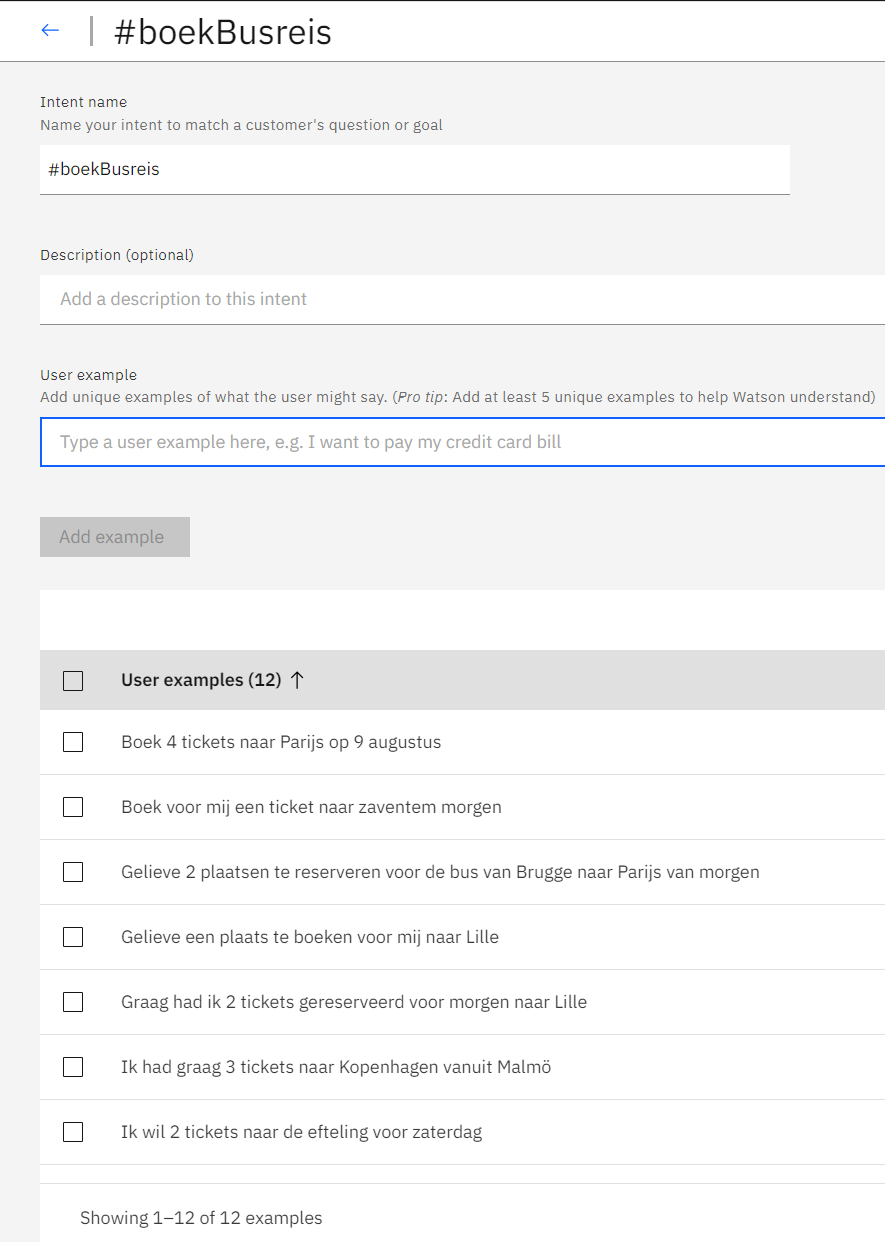
\includegraphics[width=0.75\textwidth]{watson-intent}
    \caption{Het configureren van een intent in IBM Watson}
\end{figure}

In IBM Watson kunnen ook eigen entiteiten toegevoegd worden. Dat komt vrijwel volledig overeen met hoe dat kan gedaan wordt in Dialogflow. Er kunnen waarden voor die entiteit toegevoegd worden alsook synoniemen. Het is ook mogelijk om op basis van patronen entiteiten uit berichten te halen. Het enige verschil met Dialogflow is de manier dat entiteiten gebruikt worden. Zoals eerder vermeld moet de ontwikkelaar buiten het creëren van de entiteit niets doen om het te gebruiken.

\begin{figure}[H]
    \label{fig:watson-entity}
    \centering
    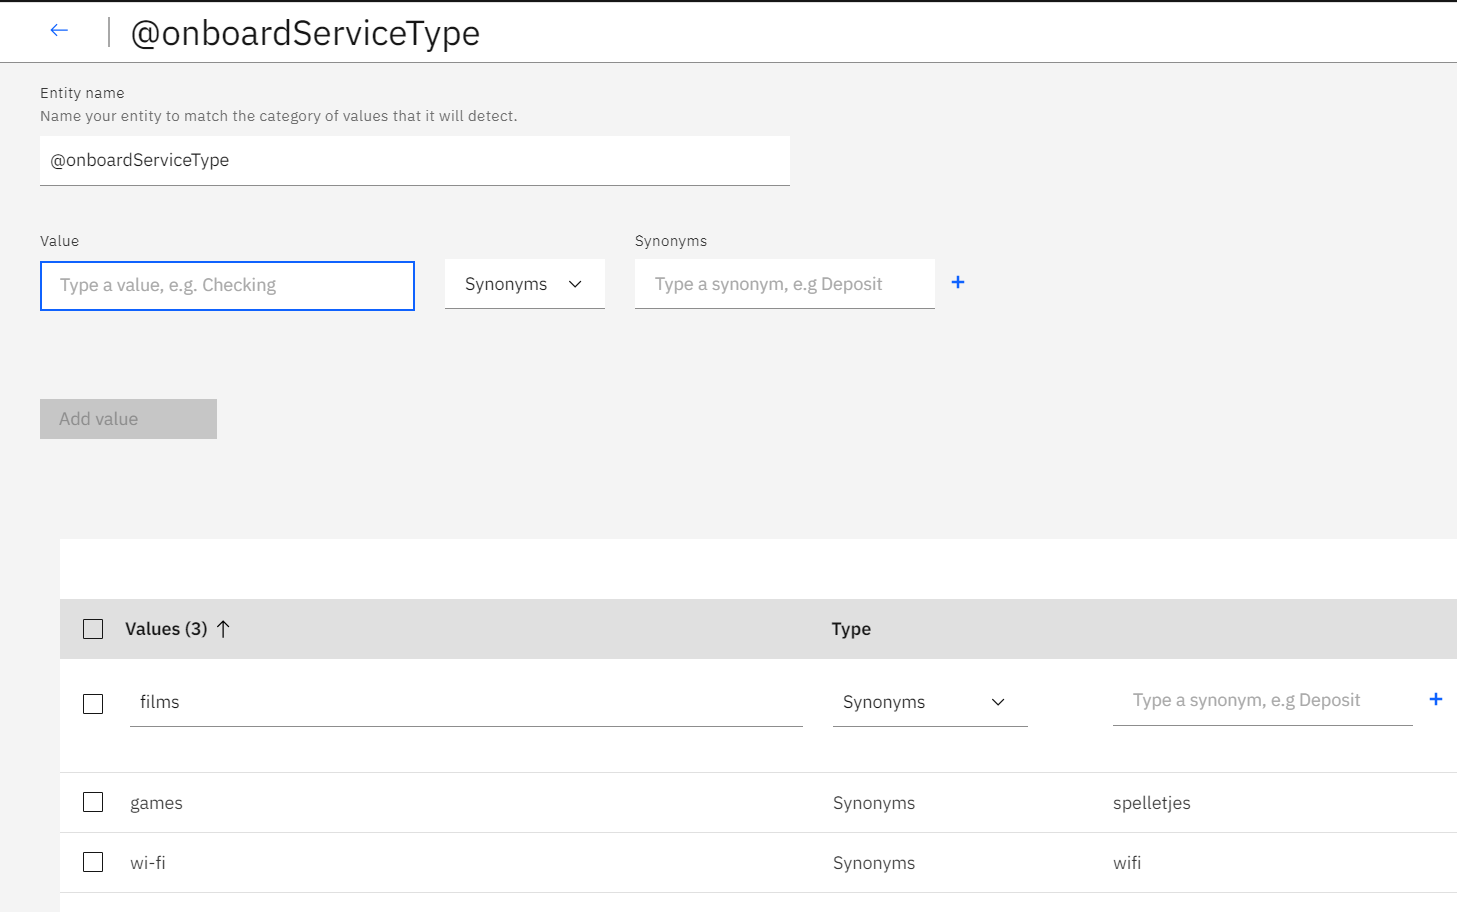
\includegraphics[width=0.9\textwidth]{watson-entity}
    \caption{Het configureren van een entiteit in IBM Watson}
\end{figure}

Het is met IBM Watson ook mogelijk om een volledige conversatieflow van een skill vast te leggen. Als ontwikkelaar kan je verschillende nodes en subnodes toevoegen en die volledig gaan configureren naar eigen wens. Deze nodes kunnen worden uitgevoerd als een intent, contextvariabele of entity herkent wordt. In de nodes kunnen er ook antwoorden voorzien worden die de assistent zal geven. Deze functionaliteit zal ook binnen deze bachelorproef niet beoordeeld worden, omdat dit geen invloed heeft op de intent classificatie prestaties van IBM Watson. Het is immers wel een interessante functionaliteit die een rol kan spelen in het kiezen naar een platform.

\begin{figure}[H]
    \label{fig:watson-dialogen}
    \centering
    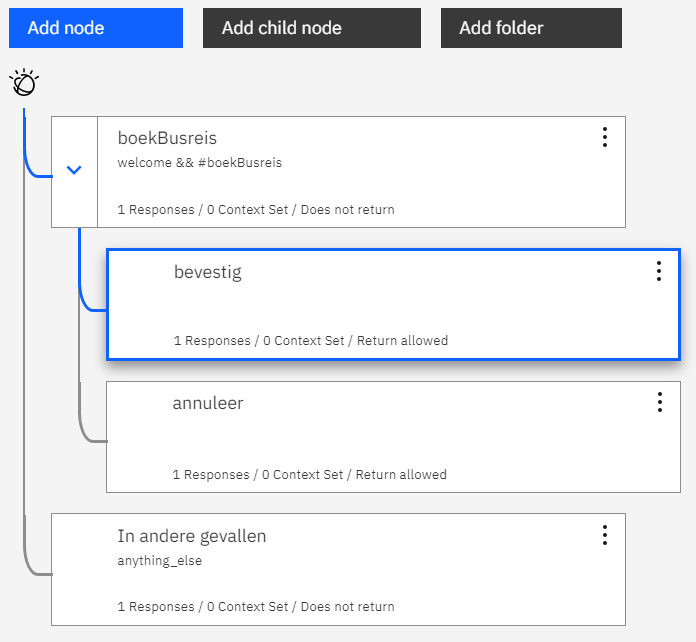
\includegraphics[width=0.75\textwidth]{watson-dialogen}
    \caption{Conversatieflow die zelf samengesteld kan worden in IBM Watson}
\end{figure}

\begin{figure}[H]
    \label{fig:watson-node}
    \centering
    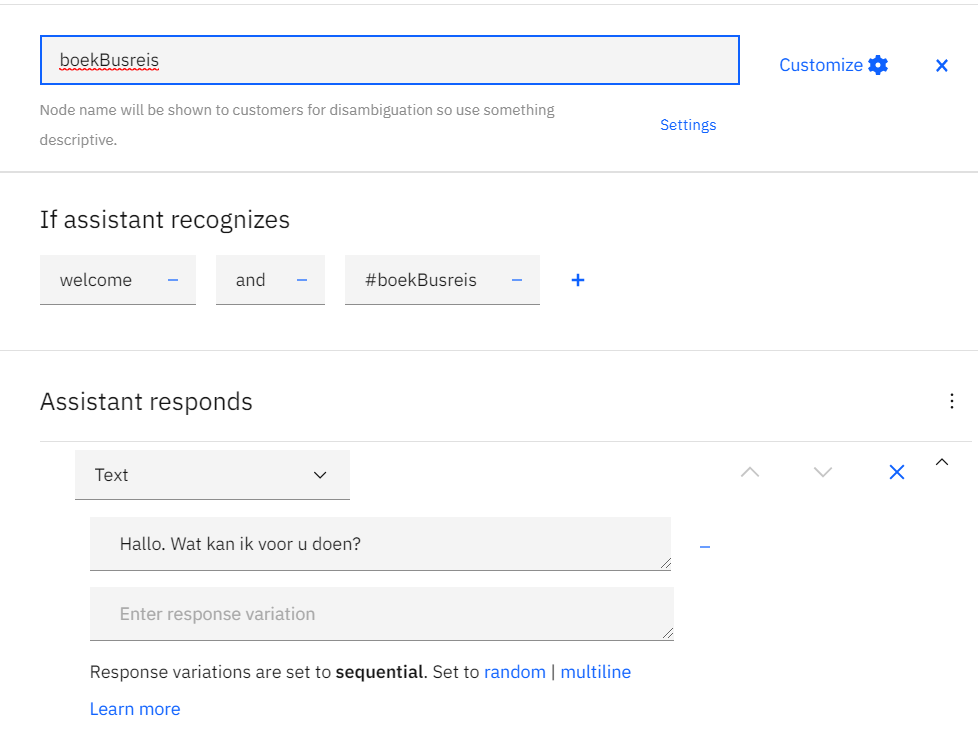
\includegraphics[width=0.75\textwidth]{watson-node}
    \caption{Het configureren van een node van in de conversatieflow in IBM Watson}
\end{figure}

Watson biedt een beperkt aantal ingebouwde integraties aan (Facebook, Slack \& eigen website), maar het is wel mogelijk om zelf een applicatie te bouwen die gebruik maakt van de aangeboden API.

De gebouwde skills kunnen ook getest worden via een ingebouwde conversatiemodule. Bij het versturen van een bericht, wordt er antwoord gegeven en is het zichtbaar welke intent herkent is.

\begin{figure}[H]
    \label{fig:watson-test}
    \centering
    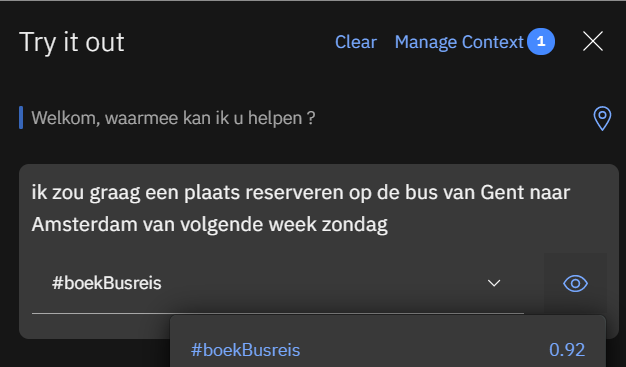
\includegraphics[width=0.65\textwidth]{watson-test}
    \caption{Het testen van IBM Watson via de ingebouwde interface}
\end{figure}

\subsection{LUIS}
\label{subsec:werking-platformen-luis}

LUIS is de NLU tool van Microsoft en is onderdeel van het Microsoft Azure cloud service platform. Dat is opnieuw goed vergelijkbaar met Google Cloud en met IBM Cloud. LUIS is een pure NLU tool, en kan dus niet worden gebruikt om dialooglogica uit te werken. Daarvoor kan het geïntegreerd worden met het Microsoft Bot Framework, die opnieuw onderdeel is van Azure en wel op berichten van eindgebruikers kan antwoorden en dialogen kan voeren. LUIS is ook onderdeel van dat framework, het wordt gewoon gezien als een individuele dienst. Het creëren van een applicatie met LUIS is ook eenvoudig doordat er een gebruiksvriendelijke interface voorzien is, net zoals alle voorgaande platformen. Om een applicatie te starten heb je enkel een Microsoft account nodig en moet je een naam en taal selecteren.

\begin{figure}[H]
    \label{fig:luis-create}
    \centering
    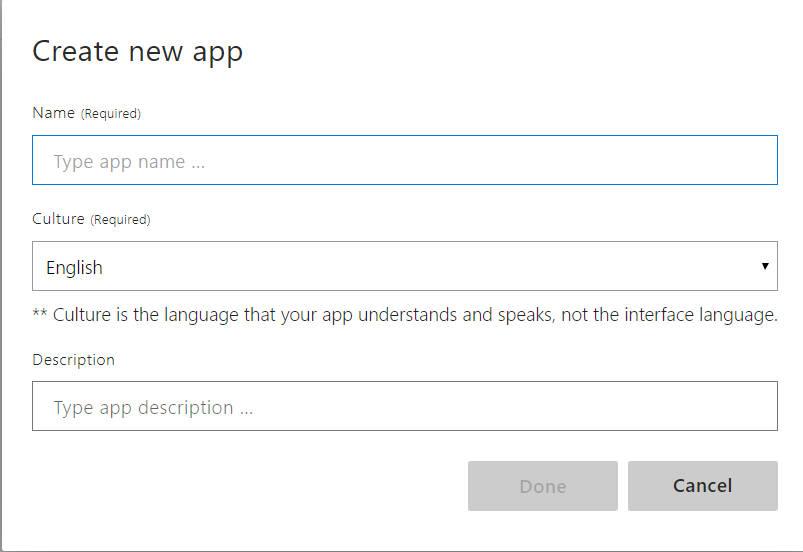
\includegraphics[width=0.65\textwidth]{luis-create}
    \caption{Het aanmaken van een applicatie via LUIS}
\end{figure}

Het toevoegen en configureren van intents is vrij gelijkaardig aan de manier die Dialogflow toepast. Het is opnieuw belangrijk dat er genoeg voorbeeldzinnen per intent zijn om er voor te zorgen dat de applicatie goed getraind kan worden. LUIS gebruikt de naam utterances om voorbeeldzinnen te beschrijven. Bij LUIS is het opnieuw vereist om zelf aan te geven welke woorden entiteiten zijn. Dit kunnen zowel systeementiteiten als zelfgemaakte entiteiten zijn.

\begin{figure}[H]
    \label{fig:luis-intent}
    \centering
    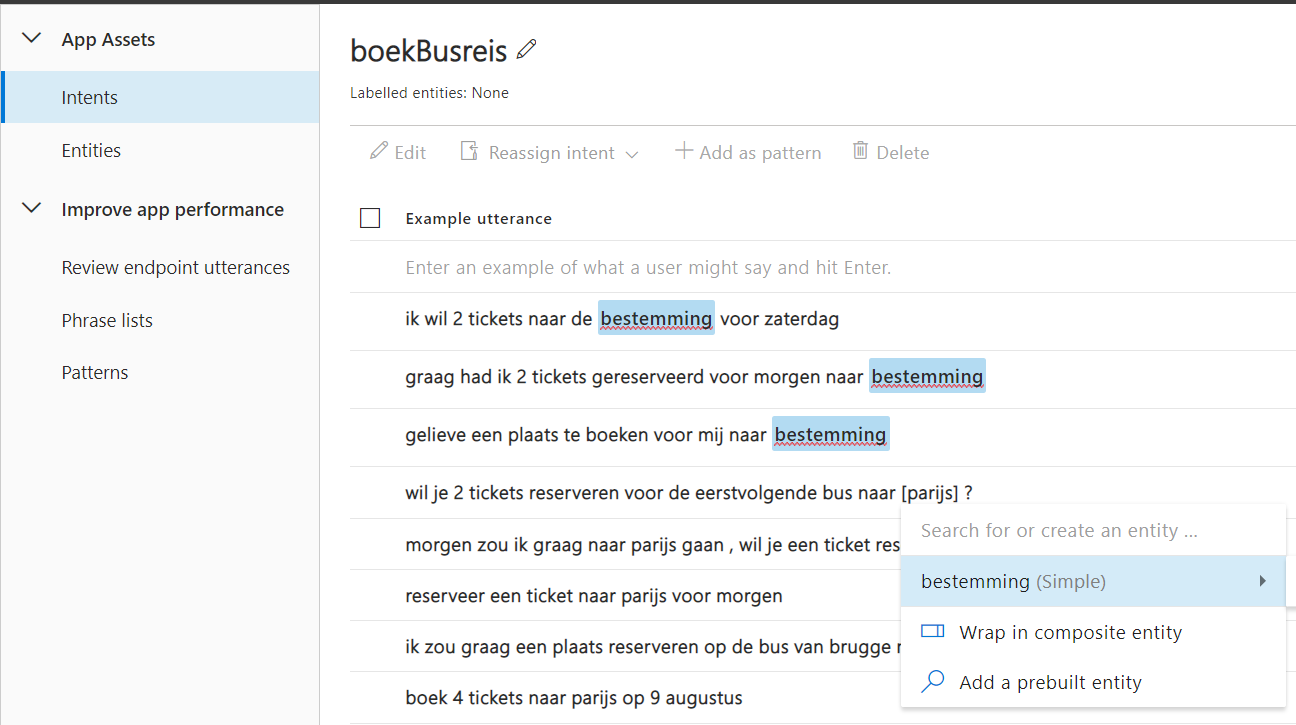
\includegraphics[width=0.85\textwidth]{luis-intent}
    \caption{Het configureren van een intent in LUIS}
\end{figure}

LUIS biedt een een grote hoeveelheid vooraf gebouwde intents, entities en zelfs domeinen aan. Domeinen zijn een verzameling van vooraf getrainde modellen van intents en entities die samenwerken. Dat kan een grote impact hebben op de prestaties van LUIS. Verder is het ook mogelijk om zelf entities toe te voegen en te gaan gebruiken. Indien je als ontwikkelaar systeementiteiten wil gebruiken, is het wel noodzakelijk om die eerst toe te voegen. Indien je dit niet doet, zal het niet mogelijk zijn om ze te gebruiken in de utterances. Er zijn verschillende soorten entiteittypes om uit te kiezen. Opvallend is wel dat er bij LUIS geen waarden voor de entiteit moeten meegegeven worden.

\begin{figure}[H]
    \label{fig:luis-entity}
    \centering
    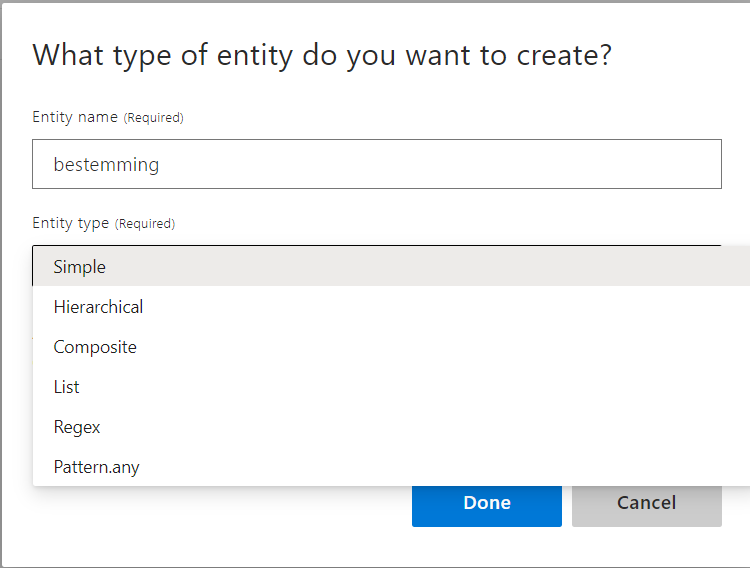
\includegraphics[width=0.65\textwidth]{luis-entity}
    \caption{Het aanmaken van een entiteit binnen LUIS}
\end{figure}

Met LUIS is het net zoals bij Dialogflow mogelijk om eerder ingevoerde data van gebruikers te gaan toewijzen of weigeren aan een specifieke intent. Het enige verschil bij LUIS is dat enkel utterances waarover hij onzeker is nog moet goedgekeurd worden.

\begin{figure}[H]
    \label{fig:luis-validate}
    \centering
    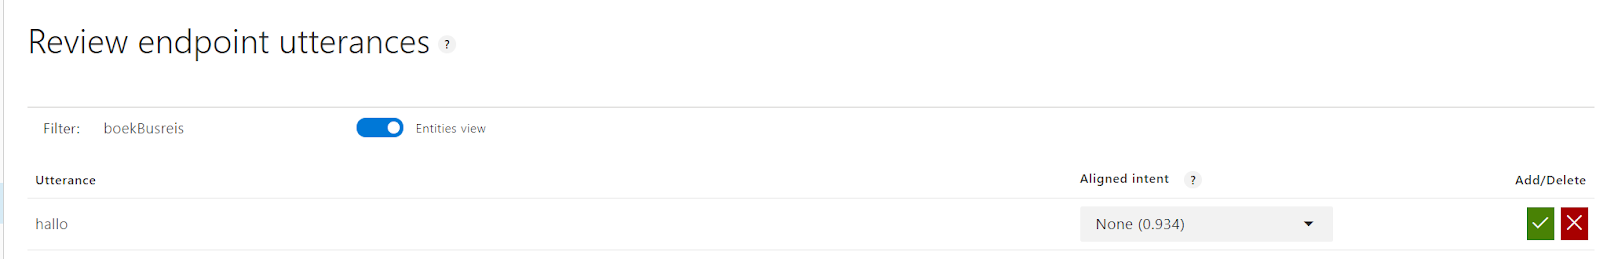
\includegraphics[width=\textwidth]{luis-validate}
    \caption{Het beoordelen van utterances waarover LUIS onzeker is}
\end{figure}

Voor LUIS kan getest worden, is het verplicht om het model te trainen. Dat moet manueel gebeuren. Indien je dit niet doet, is het gewoonweg niet mogelijk om berichten te sturen.

\begin{figure}[H]
    \label{fig:luis-train}
    \centering
    
\includegraphics[width=0.65\textwidth]{luis-train}
    \caption{Het manueel trainen van de LUIS applicatie}
\end{figure}

Eens de applicatie getraind is, kan er getest worden. Testen kan opnieuw gebeuren via een ingebouwde module. Bij het versturen van een bericht naar de gebouwde LUIS app, krijg je informatie over welke intent herkent is.
Het is ook duidelijk zichtbaar welke entities herkent zijn. Ook zal LUIS automatisch een sentimentanalyse gaan uitvoeren. Daarbij wordt aangegeven hoe positief of negatief LUIS dit bericht interpreteert.

\begin{figure}[H]
    \label{fig:luis-test}
    \centering
    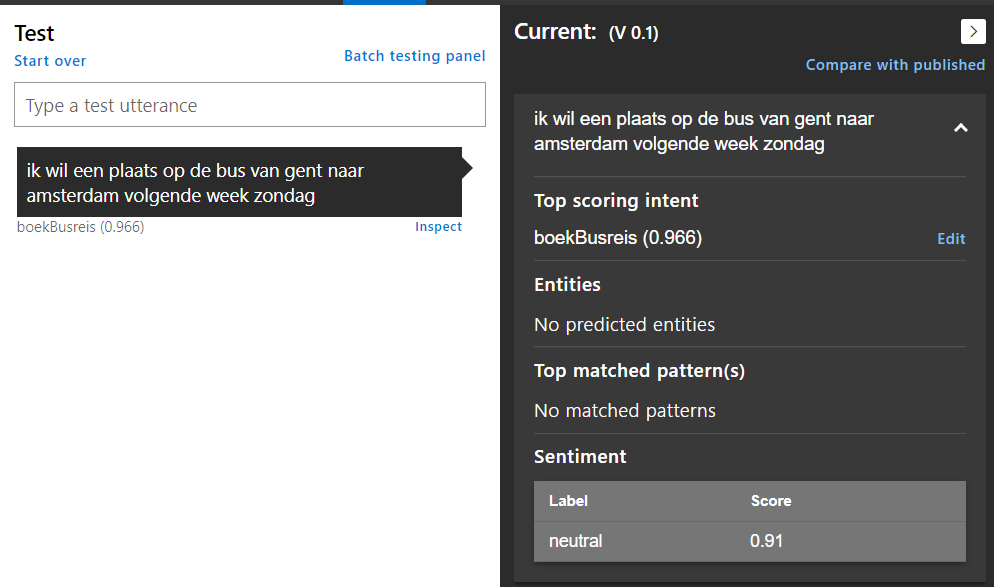
\includegraphics[width=0.75\textwidth]{luis-test}
    \caption{Het testen van een LUIS applicatie}
\end{figure}

\subsection{Wit.ai}
\label{subsec:werking-platformen-wit}

Wit.ai is de NLU tool van Facebook en is volledig gratis te gebruiken. Het heeft net zoals de vorige platformen een eenvoudige grafische user interface die gebruikt kan worden. Het enige dat je nodig hebt om aan de slag te gaan met Wit.ai is een Github account of een Facebook account. Het staat volledig gratis gehost op het internet en kan dus via de API van overal bereikt worden. Het bevat geen mogelijkheid om dialogen te configureren en antwoorden in te stellen, indien je dit wenst, moet er zelf een applicatie worden ontwikkeld die gebruik maakt van de aangeboden API.

Het aanmaken van een applicatie binnen Wit.ai is heel erg eenvoudig. Een naam en een standaardtaal is alles die nodig is. Het is ook mogelijk om een applicatie te importeren van een backup. Er is ook de keuze om de data die verwerkt wordt in de applicatie te delen met de volledige community of niet.

\begin{figure}[H]
    \label{fig:wit-create}
    \centering
    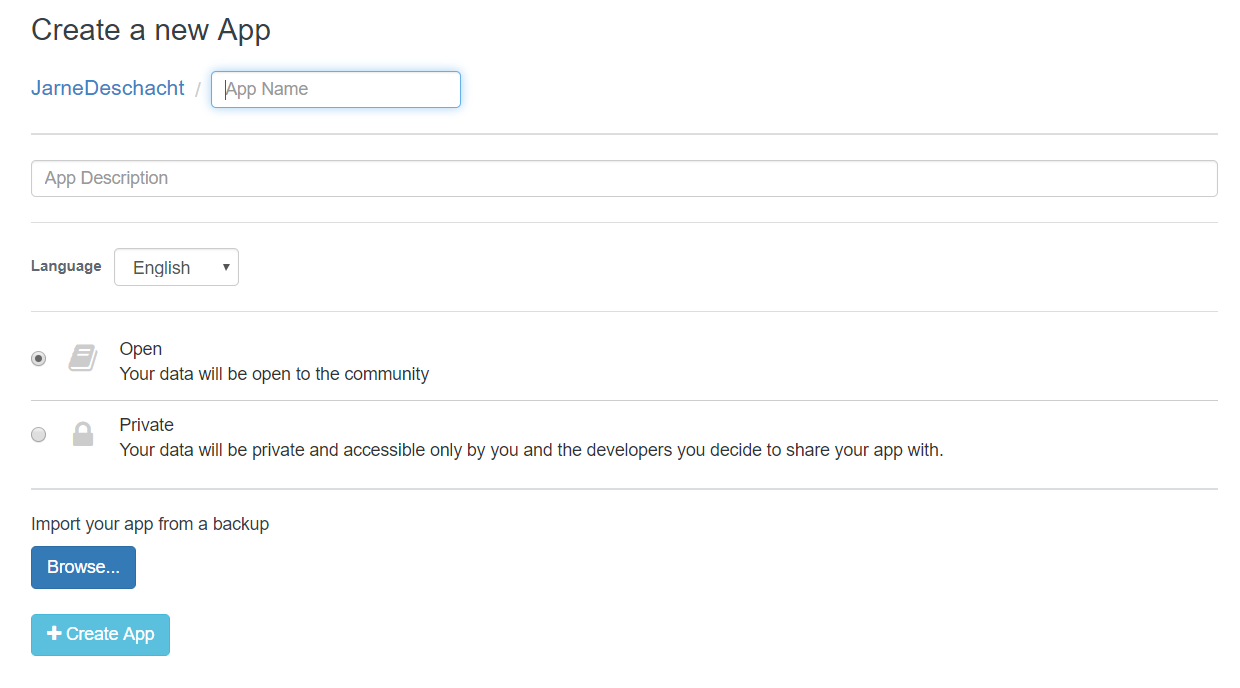
\includegraphics[width=0.75\textwidth]{wit-create}
    \caption{Het aanmaken van een applicatie in Wit.ai}
\end{figure}

Nu de applicatie aangemaakt is, kan het trainen beginnen. De werking van intents en entities binnen Wit.ai wijkt af van hoe de andere platformen hiermee omgaan. Binnen Wit.ai bestaan er enkel entities, geen intents. Intents worden gezien als een instantie van een entity. Parameterwaarden worden dus ook als entities gezien, net zoals intents. Bij het toevoegen van nieuwe trainingsdata moet dus altijd minstens één entity toegevoegd worden, namelijk de entity ‘intent’. Net zoals bij andere entities kunnen dan verschillende waarden toegevoegd worden. Deze waarden komen dan overeen met de namen van de mogelijke intents. Dit klinkt erg verwarrend, maar onderstaande voorbeelden verduidelijken deze werking.

\begin{figure}[H]
    \label{fig:wit-train}
    \centering
    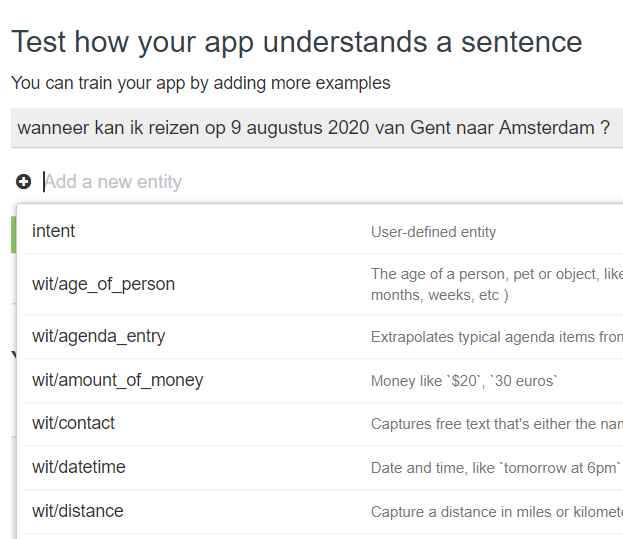
\includegraphics[width=0.65\textwidth]{wit-train}
    \caption{Het trainen van een Wit.ai applicatie}
\end{figure}

\begin{figure}[H]
    \label{fig:wit-intent}
    \centering
    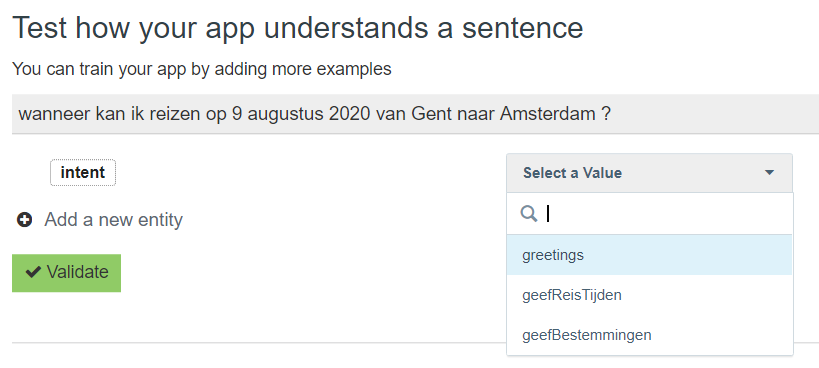
\includegraphics[width=0.65\textwidth]{wit-intent}
    \caption{Het kiezen van een intent bij het trainen in Wit.ai}
\end{figure}

Net zoals bij andere platformen is het mogelijk om extra entities toe te voegen aan voorbeeldzinnen. Er is keuze uit een aantal voorgedefinieerde entities, maar het is ook mogelijk om zelf entities aan te maken.

\begin{figure}[H]
    \label{fig:wit-entity}
    \centering
    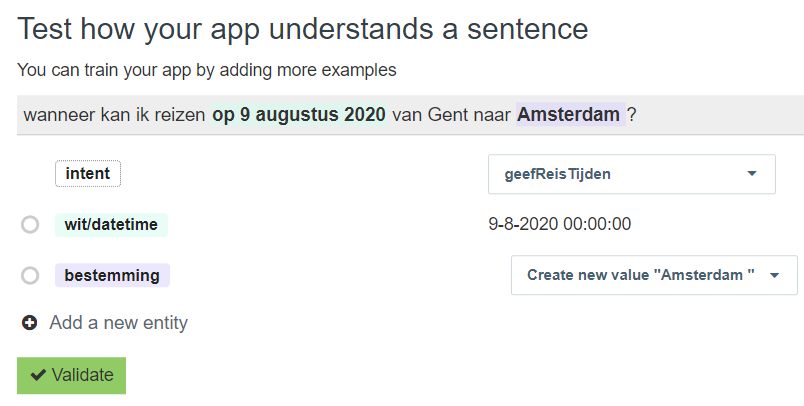
\includegraphics[width=0.65\textwidth]{wit-entity}
    \caption{Het toevoegen van extra entities aan een voorbeeldzin in Wit.ai}
\end{figure}

Het is ook mogelijk om extra waarden en synoniemen toe te voegen aan entities.

\begin{figure}[H]
    \label{fig:wit-intent-manage}
    \centering
    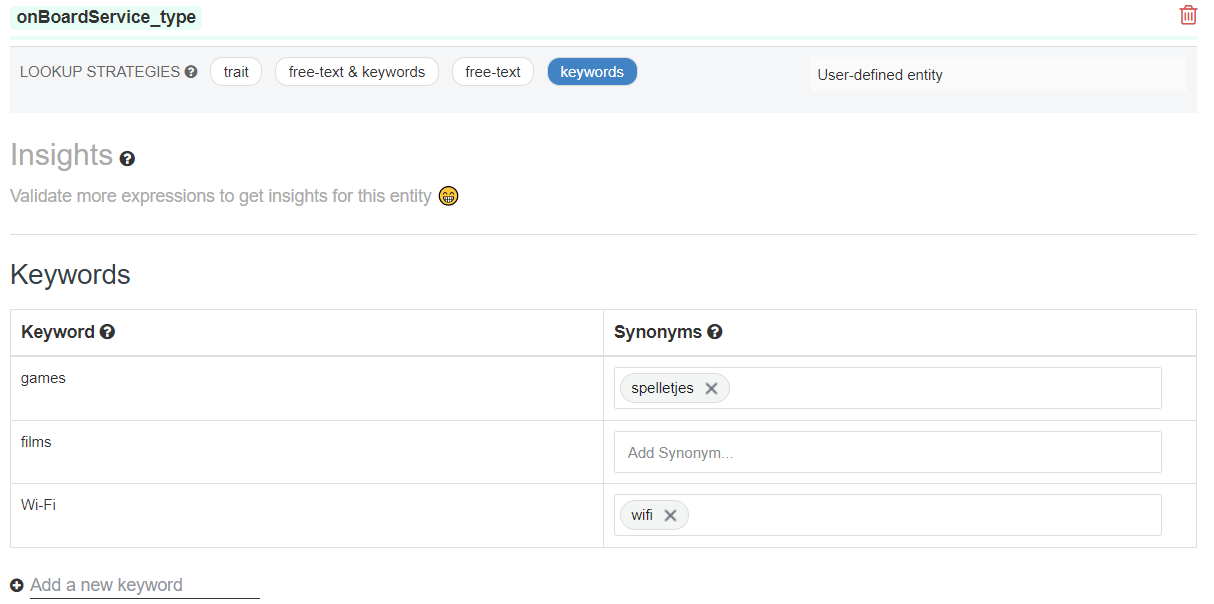
\includegraphics[width=0.85\textwidth]{wit-entity-manage}
    \caption{Het beheren van entities in Wit.ai}
\end{figure}

Wit.ai bevat geen module om de gebouwde applicaties te valideren. Het biedt wel een API aan om dat te doen. Deze API zal later ook gebruikt worden om training te automatiseren, maar meer daarover in een latere sectie. Om gebruik te maken van deze API werd een tool genaamd Postman gebruikt. Daarmee kan heel eenvoudig een verzoek naar de server van Wit.ai gestuurd worden om de chatbot te testen.

\begin{figure}[H]
    \label{fig:wit-test}
    \centering
    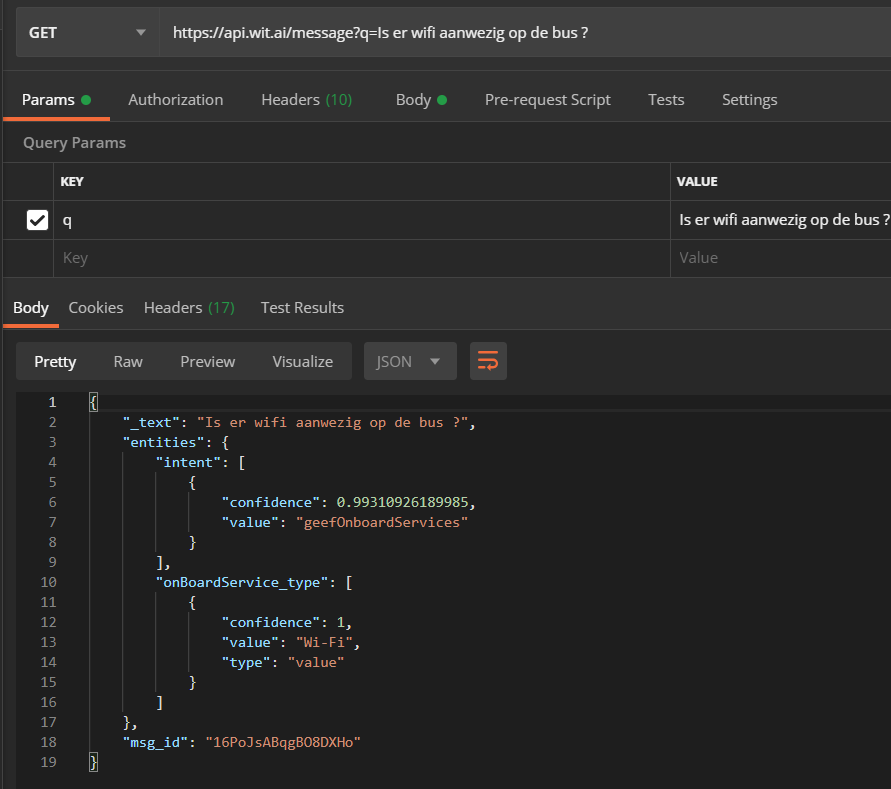
\includegraphics[width=0.75\textwidth]{wit-test}
    \caption{Voorbeeld van een request met Postman naar de server van Wit.ai om de applicatie te testen}
\end{figure}

\subsection{Rasa}
\label{subsec:werking-platformen-rasa}

Zoals eerder vermeld is Rasa een tool die qua gebruik sterk afwijkt van de eerder besproken platformen. Het vereist heel wat meer technische kennis in vergelijking met de andere. Om gebruik te maken van Rasa moet het platform eerst lokaal gedownload worden. De makkelijkste manier om dit te doen is door gebruik te maken van Pip. Pip is een tool die gebruikt wordt om softwarepakketten die geschreven zijn in de programmeertaal Python te installeren. Rasa biedt in tegenstelling tot de eerder besproken platformen ook geen grafische user interface (GUI) aan. Dat betekent dat alles in de command line interface (CLI) moet gebeuren. De CLI is de grote tegenhanger van de GUI en is een andere manier om met software te communiceren. De CLI wordt gebruikt op basis van tekstcommando's.

\begin{figure}[H]
    \label{fig:rasa-install}
    \centering
    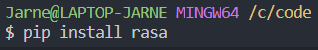
\includegraphics[width=0.35\textwidth]{rasa-install}
    \caption{Voorbeeld van een commando binnen de CLI waarbij rasa geïnstalleerd wordt door middel van Pip}
\end{figure}

Eens Rasa succesvol geïnstalleerd is, kan er een project opgestart worden. Dat kan met het commando ‘rasa init’, daarbij zal er de vraag komen in welke map het project geïnstalleerd moet worden en of dat er een voorbeeldmodel getraind moet worden. Eens dat gelukt is, kan de configuratie van de chatbot beginnen.

\begin{figure}[H]
    \label{fig:rasa-create}
    \centering
    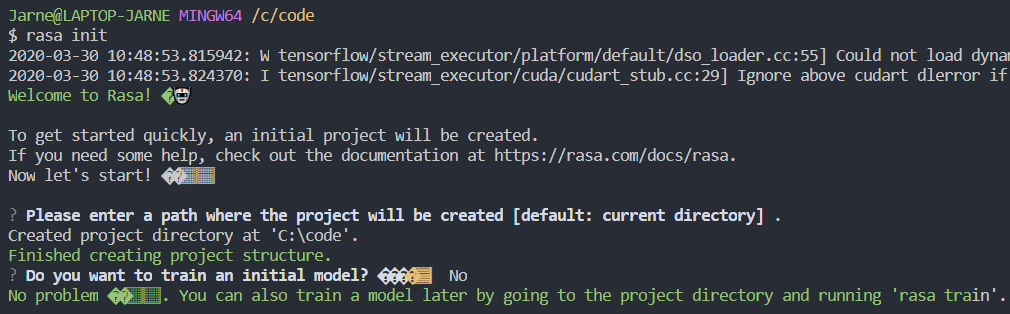
\includegraphics[width=\textwidth]{rasa-create}
    \caption{Het creëren van een project met Rasa in de CLI}
\end{figure}

Rasa bestaat uit twee hoofdmodules, Rasa NLU en Rasa Core. De focus binnen dit onderzoek zal liggen op Rasa NLU. Dit is de intent classificatiemodule van Rasa die nodig is om het begrijpend vermogen van een chatbot te evalueren. Rasa Core is essentieel voor het vastleggen van dialogen en antwoorden richting de eindgebruiker. Rasa werkt zoals de andere platformen ook met intents en entities. Het configureren ervan gebeurt in een bestand genaamd ‘nlu.md’ die aangemaakt is bij het creëren van een project. Daarin kunnen heel eenvoudig intents met bijhorende voorbeeldzinnen toegevoegd worden. Entities moeten binnen Rasa ook niet vooraf gedefinieerd worden, ze kunnen direct aangeduid worden in de voorbeeldzinnen en Rasa doet de rest. Het is ook mogelijk om synoniemen te voorzien voor entities en om entities te herkennen op basis van patronen.

\begin{figure}[H]
    \label{fig:rasa-intent}
    \centering
    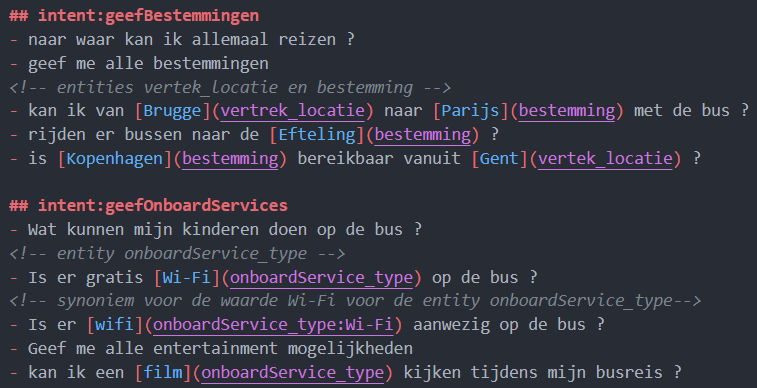
\includegraphics[width=0.85\textwidth]{rasa-intent}
    \caption{Het configureren van de intents en voorbeeldzinnen met entities in Rasa}
\end{figure}

Het moeilijkste deel bij het gebruik van Rasa is het vastleggen van de configuratie van rasa NLU en rasa Core. Rasa kan door de ontwikkelaar volledig op maat van een project afgesteld worden. Berichten die via Rasa binnenkomen worden verwerkt door softwarepakketten die je als ontwikkelaar zelf kan kiezen. Dat is iets die in de andere platformen achter de schermen voor ons wordt gedaan, dus daar hebben we niet altijd controle over. Binnen deze bachelorproef wordt er beperkt tot de nederlandse taal, dus moeten er componenten worden gebruikt die Nederlands ondersteunen. De configuratie vastleggen kan opnieuw via een bestand (config.yml) die bij het creëren aangemaakt werd. Bij het vastleggen van de configuratie werden de aanbevelingen vanuit de officiële documentatie gebruikt. Het voornaamste is dat er componenten worden gebruikt die overweg kunnen met de nederlandse taal. De configuratie van Rasa Core heeft eveneens tal van mogelijkheden, maar dit behoort niet tot de scope van deze bachelorproef. Over alle opties en mogelijkheden van Rasa kan een totaal nieuwe bachelorproef worden geschreven. 

\begin{figure}[H]
    \label{fig:rasa-config}
    \centering
    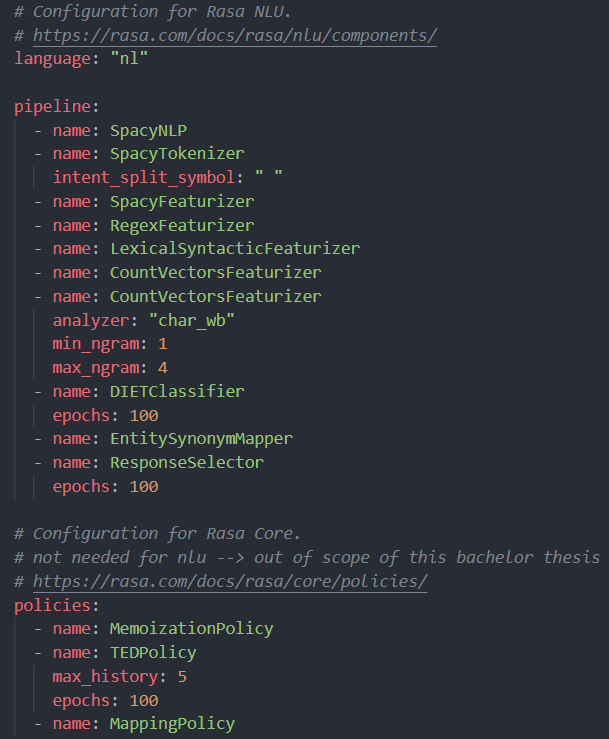
\includegraphics[width=0.55\textwidth]{rasa-config}
    \caption{Configuratie van Rasa}
\end{figure}

Met Rasa Core is het zoals eerder vermeld ook mogelijk om dialogen en antwoorden naar eindgebruikers te configureren. Rasa Core wordt standaard mee geïnstalleerd, maar zal binnen deze bachelorproef niet verder gebruikt en besproken worden.

Eens de configuratie van rasa gebeurt is en er een aantal intents toegevoegd zijn, kan het trainen en testen van de chatbot gebeuren. Het is mogelijk om afzonderlijke modules te trainen. Om enkel de NLU module te trainen moet er in de CLI het commando ‘rasa train nlu’ uitgevoerd worden.

\begin{figure}[H]
    \label{fig:rasa-train}
    \centering
    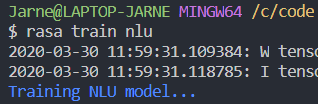
\includegraphics[width=0.5\textwidth]{rasa-train}
    \caption{Het trainen van de NLU module van Rasa}
\end{figure}

Als de training succesvol afgerond is, dan is het mogelijk om de NLU module te gaan testen. Dit kan gedaan worden door het commando ‘rasa shell nlu’ uit te voeren. Daarbij wordt een server opgestart waarnaar berichten kunnen worden gestuurd en intents en entities herkent kunnen worden. 

\begin{figure}[H]
    \label{fig:rasa-test}
    \centering
    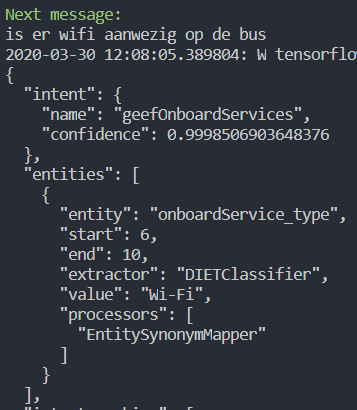
\includegraphics[width=0.5\textwidth]{rasa-test}
    \caption{Voorbeeld van een response bij het sturen van een bericht naar de NLU module}
\end{figure}

\section{Automatisatie}
\label{sec:automatisatie}

Tot nu toe werd er telkens via een user interface rechtstreeks gewerkt op de verschillende platformen om bijvoorbeeld een model te trainen of om een model te testen. Deze manier van werken is goed, maar zal bij grote hoeveelheden data heel erg veel tijd in beslag nemen. Stel je maar voor dat er 10000 voorbeeldzinnen  en 100 intents zijn en dat dit allemaal via de user interface moet ingevoerd worden. Volgens cross validation moeten er dan een aantal keer 8000 zinnen getraind worden en 2000 zinnen getest. Dit zou volgens de werking hierboven beschreven enorm veel tijd in beslag nemen en na een mum van tijd onbeheersbaar worden. Om dit op te lossen bieden de platformen een oplossing aan genaamd een API. API’s zijn een andere manier om te communiceren met de platformen. Het is mogelijk om vanuit een eigen geprogrammeerde applicatie te communiceren met deze API’s en eigenlijk van volledig dezelfde functionaliteiten gebruik te maken als hierboven beschreven zonder dat er rechtstreeks op de platformen moet gewerkt worden. Dat betekent dat we zelf code kunnen schrijven die het volledige proces van het trainen en het valideren van de platformen kan automatiseren door gebruik te maken van die API’s. Binnen deze bachelorproef werd verder enkel nog gebruik gemaakt van de verschillende API’s. Dit met het resultaat dat het experiment veel sneller uitgevoerd en herhaald kan worden zonder dat dit allemaal manueel via de user interface van de platformen moet gebeuren.
























